


\section{O`zgarmas tokning ishi va quvvati}


\begin{enumerate}

\item Energiyaning $1$ kilovatt-soat degan birligi necha Joulga teng?
\begin{enumerate}[label=\Alph*)]
\item 36 000.
\item 3600.
\item 3 600 000.
\item 100 000.
\item 1000.
\end{enumerate}

\item Talabalar yotoqxonasidagi bitta xonada quvvati $100$ W bo‘lgan elektr lampochka har kuni $6$ soatdan yonib turadi. Agar $1$ kW$\cdot$h elektr energiyasining narxi $450$ so‘m bo‘lsa, uning bir oylik ($30$ kun) harajati qancha bo‘ladi (so‘m)?
\begin{enumerate}[label=\Alph*)]
\item 5000.
\item 6500.
\item 10200.
\item 11700.
\item 8100.
\end{enumerate}

\item Tarmoqqa qanday (kW) quvvatli iste’molchi ulanganda, elektr hisoblagich diskining aylanish chastotasi $1,5$ Hz ga teng bo‘ladi? (Diskning $3000$ marta aylanishi $1$ kW$\cdot$h energiyaga mos keladi.)
\begin{enumerate}[label=\Alph*)]
\item 3.
\item 3,5.
\item 1,8.
\item 2.
\item 2,5.
\end{enumerate}

\item Elektr asbob tarmoqqa ulanganda, elektr hisoblagich diski bir minutda $30$ marta aylandi. Shu asbobning quvvati necha kW? (Hisoblagichda $1$ kW$\cdot$h diskning $1200$ aylanishiga teng deb yozilgan.)
\begin{enumerate}[label=\Alph*)]
\item 1,2.
\item 1,5.
\item 0,5.
\item 2.
\item 3.
\end{enumerate}

\item Xonaga o‘rnatilgan ventilyatorning quvvati $36$ W. Uning $20$ s da bajargan ishi qanday (J)?
\begin{enumerate}[label=\Alph*)]
\item 1,8
\item 18
\item 72
\item 360
\item 720
\end{enumerate}

\item $500$ kW quvvatga ega bo‘lgan elektrostansiya soatiga qancha ish bajarishi mumkin (MJ)?
\begin{enumerate}[label=\Alph*)]
\item 1800.
\item 3600.
\item 4000.
\item 5000.
\item 7200.
\end{enumerate}

\item Elektr quvvati $0,5$ kW bo‘lgan elektr choynak $5$ minutda qancha energiya (kJ) iste’mol qiladi?
\begin{enumerate}[label=\Alph*)]
\item 25.
\item 50.
\item 75.
\item 100.
\item 150.
\end{enumerate}

\item O‘zgarmas tokning ishi qanday formula yordamida hisoblanadi?
\begin{enumerate}[label=\Alph*)]
\item $A=IUt$.
\item $A=\dfrac{U^2}{R}$.
\item $A=IU$.
\item $A=I^2U$.
\item $A=I^2R$.
\end{enumerate}

\item Berilgan munosabatlardan qaysilari elektr toki ishini ifodalaydi?
\begin{enumerate}
\item $A=Nt$;
\item $A=Fscos\alpha$;
\item $A=q(\varphi_1-\varphi_2)$;
\item $A=IUt$;
\item $A=I^2Rt$.
\end{enumerate}
\begin{enumerate}[label=\Alph*)]
\item 3, 4, 5.
\item 1, 3, 4.
\item 1, 2, 3.
\item 1, 4.
\item 1, 3.
\end{enumerate}

\item Birligini J/(A$^2\cdot$s) ko‘rinishida yozish mumkin bo‘lgan fizik kattalik nomi nima?
\begin{enumerate}[label=\Alph*)]
\item kuchlanish.
\item o‘tkazuvchanlik.
\item tok kuchi.
\item qarshilik.
\item elektr sig‘im.
\end{enumerate}

\item Zanjirning kuchlanish $200$ V bo‘lgan qismida tok $16$ kJ ish bajargan bo‘lsa, bu qismdan nechta elektron oqib o‘tgan bo‘ladi?
\begin{enumerate}[label=\Alph*)]
\item $8\cdot10^{18}$.
\item $5\cdot10^{19}$.
\item $6,02\cdot10^{23}$.
\item $5\cdot10^{20}$.
\item $1,6\cdot10^{19}$.
\end{enumerate}

\item Agar qarshiligi $20~\Omega$ bo‘lgan o‘tkazgichning uchlariga $20$ V kuchlanish berilsa, $20$ sekundda tok necha Joul ish bajaradi?
\begin{enumerate}[label=\Alph*)]
\item 578.
\item 576.
\item 570.
\item 480.
\item 400.
\end{enumerate}

\item Zanjirning biror qismidagi kuchlanish $3$ V bo‘lganda $6$ A tok $10$ s da zanjirning shu qismida necha Joul ish bajaradi?
\begin{enumerate}[label=\Alph*)]
\item 1,8.
\item 5.
\item 20.
\item 180.
\item TJY.
\end{enumerate}

\item Zanjirning biror qismidagi kuchlanish necha Volt bo‘lganda $3$ A tok $4$ s da zanjirning shu qismida $24$ J ish bajaradi?
\begin{enumerate}[label=\Alph*)]
\item 2.
\item 0,5.
\item 32.
\item 18.
\item TJY.
\end{enumerate}

\item Elektr toki zanjirning biror qismida $3$ s da $6$ J ish bajaradi. Agar zanjir qismidagi kuchlanish $2$ V bo‘lsa, undan o‘tayotgan tokning kuchini toping (A)?
\begin{enumerate}[label=\Alph*)]
\item 1.
\item 4.
\item 9.
\item 36.
\item 12.
\end{enumerate}

\item $j^2\rho lS$ ifoda bilan aniqlanuvchi kattalikning XBS dagi birligi qanday? ($j$ -- tok zichligi, $\rho$ -- o‘tkazgichning solishtirma qarshiligi, $l$ va $S$ -- o‘tkazgichning uzunligi va ko‘ndalang kesim yuzi).
\begin{enumerate}[label=\Alph*)]
\item $\Omega$.
\item J.
\item W.
\item V.
\item A.
\end{enumerate}

\item Quyidagi ifoda orqali qaysi fizik kattalik aniqlanadi?
\[
\frac{P}{j^2\rho}
\]
$P$ -- quvvat, $j$ -- tok zichligi, $\rho$ -- solishtirma qarshilik.
\begin{enumerate}[label=\Alph*)]
\item hajm.
\item massa.
\item ish.
\item kuchlanish.
\item tok kuchi.
\end{enumerate}

\item Cho‘g‘lanma lampa balloniga $4$ V va $0,25$ A deb yozilgan. Ishlash jarayonida lampochkaning qarshiligi ($\Omega$) va quvvati (W) qanday bo‘lishini toping.
\begin{enumerate}[label=\Alph*)]
\item 12; 0,8
\item 0,25; 4
\item 16; 1
\item 6,25; 4
\item 1; 16
\end{enumerate}

\item Cho‘g‘lanma lampa sokoliga $250$ V, $25$ W deb yozilgan. Shu lampaning qarshiligi qanday ($\Omega$)?
\begin{enumerate}[label=\Alph*)]
\item 0,1
\item 10
\item 625
\item 2500
\item 6250
\end{enumerate}

\item Cho‘g‘lanma lampa balloniga $3,5$ V va $0,28$ A deb yozilgan. Lampaning ish rejimidagi qarshiligi va quvvatini topilsin.
\begin{enumerate}[label=\Alph*)]
\item 12,5 $\Omega$, 0,98 W.
\item 12,5 $\Omega$, 0,9 W.
\item 13 $\Omega$, 1 W.
\item 12 $\Omega$, 0,8 W.
\item 11 $\Omega$, 1,2 W.
\end{enumerate}

\item $72$ W quvvatli elektr chiroq $12$ V kuchlanishga mo‘ljallangan. Chiroqning qarshiligini aniqlang ($\Omega$).
\begin{enumerate}[label=\Alph*)]
\item 0,2.
\item 2.
\item 2,4.
\item 5.
\item 10.
\end{enumerate}

\item $12$ V kuchlanishga mo‘ljallangan elektr lampaning quvvati $60$ W. Lampaning qarshiligini aniqlang ($\Omega$).
\begin{enumerate}[label=\Alph*)]
\item 10.
\item 5.
\item 2,4.
\item 0,4.
\item 0,2.
\end{enumerate}

\item Elektr plitaning quvvati $1$ kW. Agar plitaning spiralidan $5$ A tok o‘tayotgan bo‘lsa, spiralning qarshiligi necha $\Omega$ ga teng?
\begin{enumerate}[label=\Alph*)]
\item 20.
\item 40.
\item 50.
\item 200.
\item 500.
\end{enumerate}

\item $1$ W quvvatga mo‘ljallangan $1~\Omega$ li rezistorga ko‘pi bilan necha Volt kuchlanish ulash mumkin?
\begin{enumerate}[label=\Alph*)]
\item 1.
\item 10.
\item 100.
\item 1000.
\item 0.
\end{enumerate}

\item $36$ V kuchlanishga mo‘ljallangan va $180$ W quvvatga ega bo‘lgan isitgich yasash uchun ko‘ndalang kesim yuzi $0,6$ mm$^2$ bo‘lgan nixrom simdan necha metr olish kerak? Nixromning solishtirma qarshiligi $\rho=1,2\cdot10^{-6}~\Omega\cdot$m.
\begin{enumerate}[label=\Alph*)]
\item 36.
\item 7,2.
\item 3,6.
\item 2,4.
\item 1,8.
\end{enumerate}

\item Tok kuchining qo‘yilgan kuchlanishga bog‘lanish grafigidan foydalanib, kuchlanish $40$ V bo‘lganda zanjirning shu qismida ajraladigan quvvatni aniqlang (W).

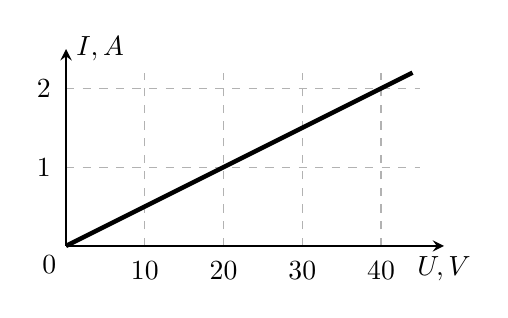
\begin{tikzpicture}[>=stealth, scale=0.1]
    % Punktir to'r (setka)
    \draw[dashed, gray!60, step=10] (0,0) grid (45, 22);

    % Koordinata o'qlari
    \draw[->, thick] (0,0) -- (48,0) node[below] {$U, \text{V}$}; % Kuchlanish o'qi
    \draw[->, thick] (0,0) -- (0,25) node[right] {$I, \text{A}$}; % Tok kuchi o'qi
    \node[below left] at (0,0) {0};

    % Grafik chizig'i (I = U/20 bog'liqligi)
    % U=20 da I=1; U=40 da I=2
    \draw[ultra thick] (0,0) -- (44, 22); 

    % Gorizontal o'qdagi (U) qiymatlar
    \node[below, yshift=-2pt] at (10,0) {10};
    \node[below, yshift=-2pt] at (20,0) {20};
    \node[below, yshift=-2pt] at (30,0) {30};
    \node[below, yshift=-2pt] at (40,0) {40};

    % Vertikal o'qdagi (I) qiymatlar
    \node[left, xshift=-2pt] at (0,10) {1};
    \node[left, xshift=-2pt] at (0,20) {2};

\end{tikzpicture}

\begin{enumerate}[label=\Alph*)]
\item 80.
\item 40.
\item 20.
\item 10.
\item $1/20$.
\end{enumerate}

\item Elektr plita tuzatilayotganda, spirali dastlabki uzunligining $0,2$ ulushiga qisqartirildi. Bunda uning quvvati qanday o‘zgaradi? $U=\text{const}$.
\begin{enumerate}[label=\Alph*)]
\item o‘zgarmaydi.
\item 1,25 marta kamayadi.
\item 1,2 marta kamayadi.
\item 1,25 marta ortadi.
\item 1,2 marta ortadi.
\end{enumerate}

\item $U_1=6$ V va $U_2=12$ V kuchlanishga mo‘ljallangan, bir xil quvvatga ega bo‘lgan ikkita lampochka qarshiliklarining nisbati $(R_1/R_2)$ nimaga teng bo‘ladi?
\begin{enumerate}[label=\Alph*)]
\item $1/4$.
\item $1/2$.
\item 1.
\item 2.
\item 4.
\end{enumerate}

\item $U_1=24$ V va $U_2=8$ V kuchlanishga mo‘ljallangan, bir xil quvvatli elektr chiroqlar qarshiliklarining nisbatini $(R_1/R_2)$ toping.
\begin{enumerate}[label=\Alph*)]
\item $1/4$.
\item $1/2$.
\item 2.
\item 4.
\item 9.
\end{enumerate}

\item Ikkita lampaning har biri $220$ V kuchlanishga mo‘ljallangan. Lampalardan birining quvvati $P_1=50$ W, boshqasiniki $P_2=150$ W. Shu lampalar qarshiliklari nisbati $R_2/R_1$ ni toping.
\begin{enumerate}[label=\Alph*)]
\item 3.
\item $1/3$.
\item 1.
\item $2/3$.
\item $3/2$.
\end{enumerate}

\item Bir xil kuchlanishga mo‘ljallangan, quvvatlari $P_1=2P_2$ bo‘lgan ikkita chiroqning qarshiliklari qanday munosabatda bo‘ladi?
\begin{enumerate}[label=\Alph*)]
\item $R_2=4R_1$.
\item $R_1=2R_2$.
\item $R_1=4R_2$.
\item $R_2=2R_1$.
\item $R_1=R_2$.
\end{enumerate}

\item Ikkita elektr isitkich tarmoqqa parallel ulangan. Birinchi isitkichning qarshiligi $50~\Omega$, ikkinchisiniki $20~\Omega$. Isitkichlar quvvatlarining nisbati $P_1/P_2$ ni toping.
\begin{enumerate}[label=\Alph*)]
\item 0,25.
\item 4.
\item 0,4.
\item 1.
\item 2.
\end{enumerate}

\item Qarshiliklari $R_1=2~\Omega$ va $R_2=8~\Omega$ bo‘lgan ikkita rezistor tok manbaiga parallel ulangan. Bu rezistorlardagi tokning quvvatlari $P_1$ va $P_2$ ni taqqoslang.
\begin{enumerate}[label=\Alph*)]
\item $P_1=2P_2$.
\item $P_1=4P_2$.
\item $P_1=P_2$.
\item $P_2=2P_1$.
\item $P_2=4P_1$.
\end{enumerate}

\item Zanjir uchlaridagi kuchlanish $1,5$ marta oshirilganda, ajralgan quvvat $6$ marta oshdi. Zanjirdan o‘tayotgan tok kuchi o‘zgardimi?
\begin{enumerate}[label=\Alph*)]
\item o‘zgarmadi.
\item 2 marta ortdi.
\item 4 marta kamaydi.
\item 4 marta ortdi.
\item 2 marta kamaydi.
\end{enumerate}

\item O‘zgarmas qarshilikka ega bo‘lgan zanjir uchlaridagi kuchlanish $6$ marta ortsa, tokning quvvati qanday o‘zgaradi?
\begin{enumerate}[label=\Alph*)]
\item o‘zgarmaydi.
\item 6 marta kamayadi.
\item 6 marta ortadi.
\item 36 marta ortadi.
\item 36 marta kamayadi.
\end{enumerate}

\item O‘tkazgich uchlaridagi kuchlanish $4$ marta ortsa, undagi tokning quvvati qanday o‘zgaradi?
\begin{enumerate}[label=\Alph*)]
\item 4 marta kamayadi.
\item 16 marta ortadi.
\item 16 marta kamayadi.
\item 4 marta ortadi.
\item o‘zgarmaydi.
\end{enumerate}

\item Kuchlanish o‘zgarmagan holda elektr qarshilik $5$ marta kamaysa, tokning quvvati qanday o‘zgaradi?
\begin{enumerate}[label=\Alph*)]
\item 25 marta ortadi.
\item o‘zgarmaydi.
\item 5 marta kamayadi.
\item 25 marta kamayadi.
\item 5 marta ortadi.
\end{enumerate}

\item Elektr tarmog‘ida qarshiliklari $100~\Omega$ va $200~\Omega$ bo‘lgan ikkita elektr lampa o‘zaro parallel ulangan. Lampalarning qaysi biri ko‘proq quvvat sarflaydi?
\begin{enumerate}[label=\Alph*)]
\item quvvat sarfi teng bo‘ladi.
\item ikkinchisi 2 marta.
\item birinchisi 2 marta.
\item ikkinchisi 4 marta.
\item birinchisi 4 marta.
\end{enumerate}

\item Kuchlanish o‘zgarmagan holda elektr qarshilik $2$ marta kamaysa, tokning quvvati qanday o‘zgaradi?
\begin{enumerate}[label=\Alph*)]
\item o‘zgarmaydi.
\item 2 marta kamayadi.
\item 2 marta ortadi.
\item 4 marta kamayadi.
\item 4 marta ortadi.
\end{enumerate}

\item Tok kuchi o‘zgarmagan holda elektr qarshilik $2$ marta kamaysa, tokning quvvati qanday o‘zgaradi?
\begin{enumerate}[label=\Alph*)]
\item o‘zgarmaydi.
\item 2 marta kamayadi.
\item 2 marta ortadi.
\item 4 marta kamayadi.
\item 4 marta ortadi.
\end{enumerate}

\item Ikkita bir xil rezistor o‘zgarmas kuchlanish tarmog‘iga avval parallel, so‘ngra ketma-ket ulandi. Qaysi holda tokning quvvati katta va necha marta katta bo‘ladi?
\begin{enumerate}[label=\Alph*)]
\item ikkala holda bir xil.
\item ketma-ket, 2 marta.
\item parallel, 2 marta.
\item ketma-ket, 4 marta.
\item parallel, 4 marta.
\end{enumerate}

\item $R_1$ rezistorda ajralayotgan quvvat $40$ W, undagi kuchlanish $10$ V, $R_2$ rezistordagi tok kuchi $2$ A, $R_3$ rezistor qarshiligi $4~\Omega$ bo‘lsa, zanjirning umumiy qarshiligi qanday ($\Omega$)?

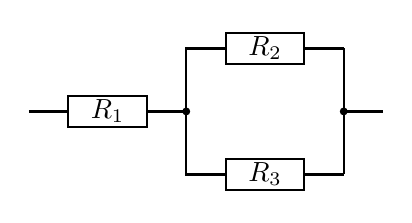
\begin{tikzpicture}[>=stealth, thick]
    % Chap tomondan kirish simi
    \draw (0,0) -- (0.5,0);

    % R1 rezistori
    \draw (0.5,-0.2) rectangle (1.5,0.2) node[midway] {$R_1$};
    \draw (1.5,0) -- (2,0);

    % Birinchi tugun (tarmoqlanish)
    \filldraw (2,0) circle (1pt);
    \draw (2,0) -- (2,0.8) -- (2.5,0.8); % Yuqori tarmoq
    \draw (2,0) -- (2,-0.8) -- (2.5,-0.8); % Pastki tarmoq

    % R2 rezistori (yuqorida)
    \draw (2.5,0.6) rectangle (3.5,1) node[midway] {$R_2$};
    \draw (3.5,0.8) -- (4,0.8);

    % R3 rezistori (pastda)
    \draw (2.5,-1) rectangle (3.5,-0.6) node[midway] {$R_3$};
    \draw (3.5,-0.8) -- (4,-0.8);

    % Ikkinchi tugun (birlashish)
    \draw (4,0.8) -- (4,-0.8);
    \filldraw (4,0) circle (1pt);
    \draw (4,0) -- (4.5,0);

\end{tikzpicture}

\begin{enumerate}[label=\Alph*)]
\item $1/3$.
\item 0,9.
\item 2.
\item 4.
\item 4,5.
\end{enumerate}

\item $U$ kuchlanish manbaiga ulangan $R$ qarshilikka $2R$ qarshilik ketma-ket ulansa, $R$ qarshilikdagi quvvat qanday o‘zgaradi?
\begin{enumerate}[label=\Alph*)]
\item 9 marta kamayadi.
\item o‘zgarmaydi.
\item 3 marta kamayadi.
\item 3 marta oshadi.
\item 2 marta kamayadi.
\end{enumerate}

\item O‘zgarmas kuchlanishga ulangan $R$ qarshilikka qanday qarshilik ketma-ket ulansa, undagi ($R$ qarshilikdagi) quvvat $2,25$ marta kamayadi?
\begin{enumerate}[label=\Alph*)]
\item $2,25R$.
\item $1,5R$.
\item $0,5R$.
\item $0,75R$.
\item $R$.
\end{enumerate}

\item Elektrodvigatel bir soatda $1080$ kJ foydali ish bajaradi va $0,4$ kW$\cdot$h energiya iste’mol qiladi. Uning FIK (%)?
\begin{enumerate}[label=\Alph*)]
\item 25.
\item 50.
\item 75.
\item 80.
\item 90.
\end{enumerate}

\item Quvvati $1$ kW bo‘lgan suv qaynatgich $5$ min da suvga $100$ kJ issiqlik miqdori uzatadi. Bu qaynatgichning FIK qanday?
\begin{enumerate}[label=\Alph*)]
\item $1/3$.
\item 114.
\item $1/5$.
\item $1/10$.
\item $1/2$.
\end{enumerate}

\item Massasi $1000$ kg bo‘lgan lift $0,025$ soatda $81$ m balandlikka tekis ko‘tarildi. Agar liftning FIK $90\%$ bo‘lsa, motor iste’mol qiladigan quvvat qanday (kW)?
\begin{enumerate}[label=\Alph*)]
\item 15.
\item 20.
\item 5.
\item 1.
\item 10.
\end{enumerate}

\item Tok kuchi $110$ A va kuchlanishi $600$ V bo‘lganda, tramvay vagoni $3$ kN tortish kuchi hosil qiladi. Agar FIK $60\%$ bo‘lsa, tramvay gorizontal yo‘lda qanday (m/s) tezlik bilan harakatlanadi?
\begin{enumerate}[label=\Alph*)]
\item 15.
\item 14.
\item 13.
\item 13,5.
\item 13,2.
\end{enumerate}

\item Elektrovoz $1,5$ kV kuchlanishli elektr tarmoqdan foydalanib, $18$ m/s tezlikda $45$ kN tortish kuchini hosil qilmoqda. Agar elektrovoz dvigatellarining FIKi $90\%$ bo‘lsa, ulardagi umumiy tok kuchi necha Amper?
\begin{enumerate}[label=\Alph*)]
\item 250.
\item 300.
\item 400.
\item 500.
\item 600.
\end{enumerate}

\item Ushbu elektr zanjirdagi 2-dazmolning quvvatini toping (W).

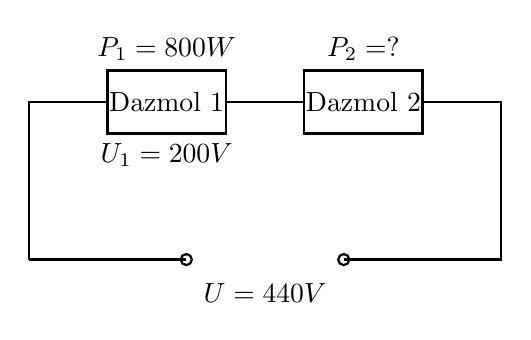
\begin{tikzpicture}[>=stealth, thick]
    % Elektr zanjiri asosi (to'rtburchak)
    \draw (0,0) -- (0,2) -- (1,2);
    \draw (5,2) -- (6,2) -- (6,0) -- (4,0);
    \draw (2,0) -- (0,0);

    % Manba (Source) pastda
    \draw (2,0) circle (2pt);
    \draw (4,0) circle (2pt);
    \node[below, yshift=-5pt] at (3,0) {$U = 440 \text{ V}$};

    % 1-dazmol (Iron 1)
    \draw (1,1.6) rectangle (2.5,2.4);
    \node at (1.75,2) {Dazmol 1};
    \node[above] at (1.75,2.4) {$P_1 = 800 \text{ W}$};
    \node[below] at (1.75,1.6) {$U_1 = 200 \text{ V}$};

    % Bog'lovchi sim
    \draw (2.5,2) -- (3.5,2);

    % 2-dazmol (Iron 2)
    \draw (3.5,1.6) rectangle (5,2.4);
    \node at (4.25,2) {Dazmol 2};
    \node[above] at (4.25,2.4) {$P_2 = ?$};

\end{tikzpicture}
\begin{enumerate}[label=\Alph*)]
\item 150.
\item 100.
\item 220.
\item 1200.
\item 960.
\end{enumerate}

\item Agar sxemadagi $K$ kalit ulansa zanjirda ajralib chiqayotgan quvvat qanday o‘zgaradi?

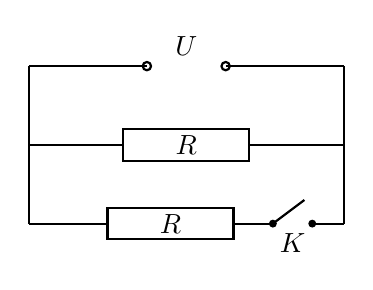
\begin{tikzpicture}[>=stealth, thick]
    % Kuchlanish manbai (U) yuqorida
    \draw (1,2) -- (2.5,2);
    \draw (3.5,2) -- (5,2);
    \draw (2.5,2) circle (1.5pt);
    \draw (3.5,2) circle (1.5pt);
    \node[above] at (3,2) {$U$};

    % Yon tarmoqlar
    \draw (1,2) -- (1,0);
    \draw (5,2) -- (5,0);

    % Birinchi (yuqori) parallel tarmoq - R rezistori
    \draw (1,1) -- (2.2,1);
    \draw (2.2,0.8) rectangle (3.8,1.2) node[midway] {$R$};
    \draw (3.8,1) -- (5,1);

    % Ikkinchi (pastki) parallel tarmoq - R rezistori va K kaliti
    \draw (1,0) -- (2,0);
    \draw (2,-0.2) rectangle (3.6,0.2) node[midway] {$R$};
    \draw (3.6,0) -- (4.1,0);
    
    % K kalitining tasviri (ochiq holatda)
    \draw (4.1,0) -- (4.5, 0.3); 
    \filldraw (4.1,0) circle (1pt);
    \filldraw (4.6,0) circle (1pt);
    \node[below] at (4.35,0) {$K$};
    \draw (4.6,0) -- (5,0);

\end{tikzpicture}
\begin{enumerate}[label=\Alph*)]
\item o‘zgarmaydi.
\item 2 marta kamayadi.
\item 4 marta kamayadi.
\item 4 marta ortadi.
\item 2 marta ortadi.
\end{enumerate}

\item Rasmda kuchlanish manbaiga ulangan $4$ ta lampochka tasvirlangan. Qaysi lampochkada eng katta quvvat ajraladi? Agar $U=100$ V bo‘lsa, shu quvvatni toping.

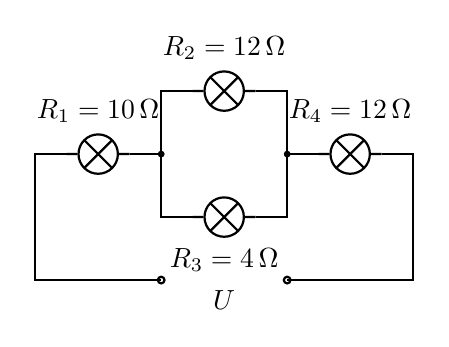
\begin{tikzpicture}[scale=0.8, >=stealth, thick, 
    bulb/.style={circle, draw, minimum size=0.5cm, inner sep=0pt, 
    path picture={\draw (path picture bounding box.south west) -- (path picture bounding box.north east) 
    (path picture bounding box.north west) -- (path picture bounding box.south east);}}]
    
    % Kuchlanish manbai (U) va asosiy simlar
    \draw (1,0) -- (0,0) -- (0,2) -- (0.5,2);
    \draw (5.5,2) -- (6,2) -- (6,0) -- (5,0);
    \draw (2,0) circle (1.5pt);
    \draw (4,0) circle (1.5pt);
    \node[below] at (3,0) {$U$};
    \draw (1,0) -- (2,0);
    \draw (4,0) -- (5,0);

    % 1-lampochka (R1)
    \node[bulb, label=above:{$R_1=10 \, \Omega$}] (L1) at (1,2) {};
    \draw (0.5,2) -- (L1) -- (1.5,2);

    % Tarmoqlanish (Parallel blok boshi)
    \draw (1.5,2) -- (2,2);
    \filldraw (2,2) circle (1pt);
    \draw (2,2) -- (2,3) -- (2.5,3);
    \draw (2,2) -- (2,1) -- (2.5,1);

    % 2- va 3-lampochkalar (Parallel tarmoqlar)
    \node[bulb, label=above:{$R_2=12 \, \Omega$}] (L2) at (3,3) {};
    \node[bulb, label=below:{$R_3=4 \, \Omega$}] (L3) at (3,1) {};
    
    \draw (2.5,3) -- (L2) -- (3.5,3);
    \draw (2.5,1) -- (L3) -- (3.5,1);

    % Birlashish (Parallel blok oxiri)
    \draw (3.5,3) -- (4,3) -- (4,2);
    \draw (3.5,1) -- (4,1) -- (4,2);
    \filldraw (4,2) circle (1pt);
    \draw (4,2) -- (4.5,2);

    % 4-lampochka (R4)
    \node[bulb, label=above:{$R_4=12 \, \Omega$}] (L4) at (5,2) {};
    \draw (4.5,2) -- (L4) -- (5.5,2);

\end{tikzpicture}

\begin{enumerate}[label=\Alph*)]
\item 1-lampochkada 160 W.
\item 3-lampochkada 2500 W.
\item 4-lampochkada 192 W.
\item 2- va 4-lampochkada bir xil 250 W.
\item 1- va 3-lampochkada bir xil 180 W.
\end{enumerate}

\item Chizmada berilgan zanjirdagi elektr tokining quvvati qanday (W). $U=12$ V, $R_1=7~\Omega$, $R_2=5~\Omega$, $R_3=R_5=4~\Omega$, $R_4=9~\Omega$.

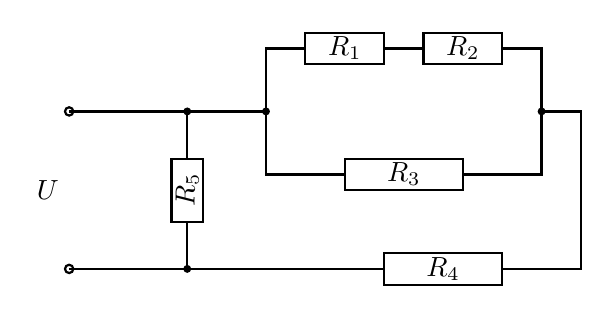
\begin{tikzpicture}[>=stealth, thick]
    % Kuchlanish manbai terminallari (U)
    \draw (0,2) circle (1.5pt);
    \draw (0,0) circle (1.5pt);
    \node[left] at (0,1) {$U$};
    
    % Kirish simlari
    \draw (0,2) -- (1.5,2);
    \draw (0,0) -- (1.5,0);

    % R5 rezistori (vertikal ulanish)
    \draw (1.5,2) -- (1.5,1.4);
    \draw (1.3,0.6) rectangle (1.7,1.4) node[midway, rotate=90] {$R_5$};
    \draw (1.5,0.6) -- (1.5,0);
    \filldraw (1.5,2) circle (1pt);
    \filldraw (1.5,0) circle (1pt);

    % Parallel blok boshlanishi
    \draw (1.5,2) -- (2.5,2);
    \filldraw (2.5,2) circle (1pt);

    % Yuqori tarmoq: R1 va R2 ketma-ket
    \draw (2.5,2) -- (2.5,2.8) -- (3,2.8);
    \draw (3,2.6) rectangle (4,3) node[midway] {$R_1$};
    \draw (4,2.8) -- (4.5,2.8);
    \draw (4.5,2.6) rectangle (5.5,3) node[midway] {$R_2$};
    \draw (5.5,2.8) -- (6,2.8) -- (6,2);

    % Pastki tarmoq: R3 rezistori
    \draw (2.5,2) -- (2.5,1.2) -- (3.5,1.2);
    \draw (3.5,1) rectangle (5,1.4) node[midway] {$R_3$};
    \draw (5,1.2) -- (6,1.2) -- (6,2);
    \filldraw (6,2) circle (1pt);

    % R4 rezistori (pastki qaytish simida)
    \draw (6,2) -- (6.5,2) -- (6.5,0) -- (5.5,0);
    \draw (4,-0.2) rectangle (5.5,0.2) node[midway] {$R_4$};
    \draw (4,0) -- (1.5,0);

\end{tikzpicture}

\begin{enumerate}[label=\Alph*)]
\item 40.
\item 36.
\item 48.
\item 42.
\item 24.
\end{enumerate}

\end{enumerate}

\begin{table}[h!]
\centering
\begin{tabular}{|c|c|c|c|c|c|c|c|c|c|}
\hline
1c & 2e & 3c & 4b & 5e & 6a & 7e & 8a & 9a & 10d \\ \hline
11d & 12d & 13d & 14a & 15a & 16c & 17a & 18c & 19d & 20a \\ \hline
21b & 22c & 23b & 24a & 25c & 26a & 27d & 28e & 29e & 30b \\ \hline
31d & 32b & 33b & 34d & 35d & 36b & 37e & 38b & 39c & 40b \\ \hline
41e & 42e & 43a & 44c & 45c & 46a & 47e & 48e & 49e & 50e \\ \hline
 51e & 52c & 53c &  &  &  &  & & &  \\ \hline
\end{tabular}
\end{table}











\section{Joul Lens qonuni}


\begin{enumerate}

\item Berilgan formulalardan qaysi biri Joul-Lens qonunini ifodalaydi?
\begin{enumerate}[label=\Alph*)]
\item $Q=I^2Rt$.
\item $Q=\lambda m$.
\item $Q=cm(t_2-t_1)$.
\item $Q=A+\Delta U$.
\item $Q=\lambda m$.
\end{enumerate}

\item O‘tkazgichdan tok o‘tganda ajralib chiqadigan issiqlik miqdori quyidagi ifodalarning qaysi biri asosida hisoblanadi?
\begin{enumerate}[label=\Alph*)]
\item $Q=cm(t_2-t_1)$.
\item $Q=IU$.
\item $Q=\dfrac{U^2}{I}$.
\item $Q=I^2Rt$.
\item $Q=Irt$.
\end{enumerate}

\item Qarshiligi $2~\Omega$ bo‘lgan simdan $15$ A tok o‘tadi. $2$ minut ichida undan qancha energiya ajraladi (kJ)?
\begin{enumerate}[label=\Alph*)]
\item 27.
\item 54.
\item 450.
\item 900.
\item 6.
\end{enumerate}

\item $50~\Omega$ qarshilikli o‘tkazgich orqali $10$ minut davomida qanday tok o‘tkazilganda, $120$ kJ issiqlik ajralib chiqadi (A)?
\begin{enumerate}[label=\Alph*)]
\item 2.
\item 3.
\item 4.
\item 5.
\item 10.
\end{enumerate}

\item Qarshiligi $12~\Omega$ bo‘lgan o‘tkazgich $120$ V kuchlanishli tarmoqqa ulangan. O‘tkazgichdan $10$ min ichida qancha issiqlik ajraladi?
\begin{enumerate}[label=\Alph*)]
\item 72 kJ.
\item 72 J.
\item 0,72 kJ.
\item 720 kJ.
\item 7,2 MJ.
\end{enumerate}

\item Tok kuchi necha amper bo‘lganda zanjirning qarshiligi $2~\Omega$ bo‘lgan qismida $3$ s da $54$ J issiqlik ajraladi?
\begin{enumerate}[label=\Alph*)]
\item 18.
\item 9.
\item 3.
\item 6.
\item TJY.
\end{enumerate}

\item Uchlaridagi kuchlanish $3$ V bo‘lgan qo‘zg‘almas o‘tkazgichdan $12$ C zaryad o‘tganda necha Joul issiqlik ajralib chiqadi?
\begin{enumerate}[label=\Alph*)]
\item 0,25.
\item 2.
\item 4.
\item 36.
\item 108.
\end{enumerate}

\item Qo‘zg‘almas o‘tkazgichdan $2$ C zaryad o‘tganda $10$ J issiqlik ajralib chiqdi. O‘tkazgich uchlaridagi kuchlanish necha Volt?
\begin{enumerate}[label=\Alph*)]
\item 0,2.
\item 2,5.
\item 5.
\item 20.
\item 40.
\end{enumerate}

\item Tok kuchi $5$ A bo‘lganda, elektr plitaning qizishi uchun $30$ minut davomida $1080$ kJ energiya sarflandi. Plitaning qarshiligini hisoblang ($\Omega$).
\begin{enumerate}[label=\Alph*)]
\item 24.
\item 26.
\item 28.
\item 30.
\item 32.
\end{enumerate}

\item Agar $1$ l suvni isitish uchun $70~\Omega$ qarshilikli o‘tkazgichdan $5$ A tok $2$ minut davomida o‘tganda ajralgan issiqlikning hammasi sarflangan bo‘lsa, suvning temperaturasi necha gradusga ko‘tarilgan? Suvning solishtirma issiqlik sig‘imi $4,2$ kJ/(kg$\cdot$K).
\begin{enumerate}[label=\Alph*)]
\item 50.
\item 60.
\item 70.
\item 80.
\item 40.
\end{enumerate}

\item Elektr plita spiralining uzunligini $2$ marta kamaytirsak, ajralib chiqayotgan issiqlik miqdori o‘zgaradimi? $U=\text{const}$.
\begin{enumerate}[label=\Alph*)]
\item 2 marta kamayadi.
\item 4 marta oshadi.
\item o‘zgarmaydi.
\item 4 marta kamayadi.
\item 2 marta oshadi.
\end{enumerate}

\item Elektr zanjir solishtirma qarshiliklari $\rho_1$ va $\rho_2$ bo‘lgan materiallardan tuzilgan, bir xil kesimli, lekin har xil $l_1$ va $l_2$ uzunlikli sim bo‘laklaridan tuzilgan. Simlar ketma-ket ulanib, tok manbaiga ulangan. Simlarda ajralayotgan issiqlik bir xil ekanligi ma’lum. Simlarning uzunliklari va qarshiliklari orasidagi munosabatni toping?
\begin{enumerate}[label=\Alph*)]
\item $\dfrac{l_1+l_2}{l_1-l_2}=\dfrac{\rho_2+\rho_1}{\rho_2-\rho_1}$.
\item $\dfrac{l_1}{l_2}=\dfrac{\rho_1}{\rho_2}$.
\item $l_1=l_2,\ \rho_1=\rho_2$.
\item $\dfrac{l_1}{l_2}=\dfrac{\rho_2}{\rho_1}$.
\item $\dfrac{l_1+l_2}{l_2}=\dfrac{\rho_2+\rho_1}{\rho_2}$.
\end{enumerate}

\item Qarshiliklari $5~\Omega$ va $10~\Omega$ bo‘lgan ikkita o‘tkazgich zanjirga ketma-ket ulangan. Birinchi o‘tkazgichda $100$ J issiqlik ajralib chiqqan vaqt ichida ikkinchi o‘tkazgichda necha kJ issiqlik ajralib chiqadi?
\begin{enumerate}[label=\Alph*)]
\item 0,1.
\item 0,2.
\item 0,4.
\item 0,5.
\item 1.
\end{enumerate}

\item Qarshiliklari $150~\Omega$ va $90~\Omega$ bo‘lgan rezistorlar tok manbaiga ketma-ket ulangan. Ikkinchi rezistorda $18$ kJ issiqlik ajralganda, birinchi rezistorda necha kJ issiqlik ajraladi?
\begin{enumerate}[label=\Alph*)]
\item 10.
\item 20.
\item 30.
\item 90.
\item 150.
\end{enumerate}

\item Qarshiliklari $R_1=20~\Omega$ va $R_2=60~\Omega$ bo‘lgan spirallar o‘zgarmas tok manbaiga ketma-ket ulangan. Bu spirallardan bir xil vaqt davomida ajralgan issiqlik miqdorlari $Q_1$ va $Q_2$ ni taqqoslang.
\begin{enumerate}[label=\Alph*)]
\item $Q_1=9Q_2$.
\item $Q_1=3Q_2$.
\item $Q_1=Q_2$.
\item $Q_2=3Q_1$.
\item $Q_2=9Q_1$.
\end{enumerate}

\item Zanjirning birinchi, ikkinchi va uchinchi qismlarida vaqt birligida ajraluvchi $Q_1$, $Q_2$ va $Q_3$ issiqlik miqdorlari orasidagi munosabatni ko‘rsating. (hamma qarshiliklar bir xil).

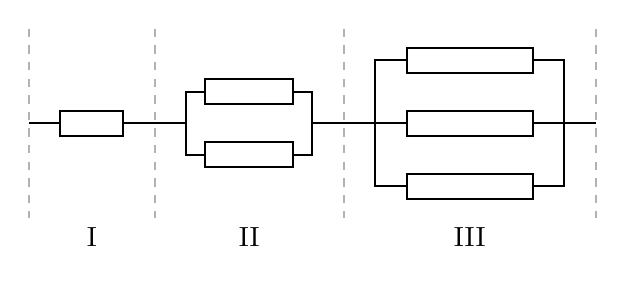
\begin{tikzpicture}[>=stealth, thick, scale=0.8]
    % Bo'limlarni ajratuvchi punktir chiziqlar
    \draw[dashed, gray!60] (-0.5, 1.5) -- (-0.5, -1.5);
    \draw[dashed, gray!60] (1.5, 1.5) -- (1.5, -1.5);
    \draw[dashed, gray!60] (4.5, 1.5) -- (4.5, -1.5);
    \draw[dashed, gray!60] (8.5, 1.5) -- (8.5, -1.5);

    % Rim raqamlari (I, II, III)
    \node at (0.5, -1.8) {I};
    \node at (3, -1.8) {II};
    \node at (6.5, -1.8) {III};

    % I-qism: Bitta rezistor
    \draw (-0.5, 0) -- (0, 0);
    \draw (0, -0.2) rectangle (1, 0.2);
    \draw (1, 0) -- (1.5, 0);

    % II-qism: Ikkita parallel rezistor
    \draw (1.5, 0) -- (2, 0);
    \draw (2, 0) -- (2, 0.5) -- (2.3, 0.5);
    \draw (2, 0) -- (2,-0.5) -- (2.3,-0.5);
    \draw (2.3, 0.3) rectangle (3.7, 0.7);
    \draw (2.3, -0.7) rectangle (3.7, -0.3);
    \draw (3.7, 0.5) -- (4, 0.5) -- (4, 0);
    \draw (3.7, -0.5) -- (4, -0.5) -- (4, 0);
    \draw (4, 0) -- (4.5, 0);

    % III-qism: Uchta parallel rezistor
    \draw (4.5, 0) -- (5, 0);
    \draw (5, 0) -- (5, 1) -- (5.5, 1);
    \draw (5, 0) -- (5.5, 0);
    \draw (5, 0) -- (5, -1) -- (5.5, -1);
    \draw (5.5, 0.8) rectangle (7.5, 1.2);
    \draw (5.5, -0.2) rectangle (7.5, 0.2);
    \draw (5.5, -1.2) rectangle (7.5, -0.8);
    \draw (7.5, 1) -- (8, 1) -- (8, 0);
    \draw (7.5, 0) -- (8, 0);
    \draw (7.5, -1) -- (8, -1) -- (8, 0);
    \draw (8, 0) -- (8.5, 0);

\end{tikzpicture}
\begin{enumerate}[label=\Alph*)]
\item $Q_1=Q_2=Q_3$.
\item $Q_1=Q_2/4=Q_3/9$.
\item $Q_1=4Q_2=9Q_3$.
\item $Q_1=Q_2/2=Q_3/3$.
\item $Q_1=2Q_2=3Q_3$.
\end{enumerate}

\item Agar $R_1=R_2=R_3$ bo‘lsa, rezistorlardan bir xil vaqt davomida ajralib chiqayotgan issiqliklarning nisbati $Q_1:Q_2:Q_3$ ni aniqlang.

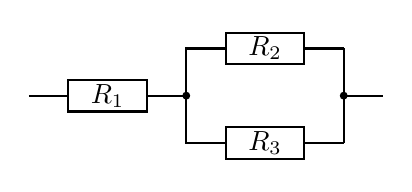
\begin{tikzpicture}[>=stealth, thick]
    % Chap tomondan kirish simi
    \draw (0,0) -- (0.5,0);

    % R1 rezistori (asosiy zanjirda)
    \draw (0.5,-0.2) rectangle (1.5,0.2) node[midway] {$R_1$};
    \draw (1.5,0) -- (2,0);

    % Birinchi tugun (parallel tarmoqlanish boshlanishi)
    \filldraw (2,0) circle (1pt);
    \draw (2,0) -- (2,0.6) -- (2.5,0.6); % Yuqori tarmoqqa
    \draw (2,0) -- (2,-0.6) -- (2.5,-0.6); % Pastki tarmoqqa

    % R2 rezistori (yuqori tarmoqda)
    \draw (2.5,0.4) rectangle (3.5,0.8) node[midway] {$R_2$};
    \draw (3.5,0.6) -- (4,0.6);

    % R3 rezistori (pastki tarmoqda)
    \draw (2.5,-0.8) rectangle (3.5,-0.4) node[midway] {$R_3$};
    \draw (3.5,-0.6) -- (4,-0.6);

    % Ikkinchi tugun (parallel tarmoqlanish tugashi)
    \draw (4,0.6) -- (4,-0.6);
    \filldraw (4,0) circle (1pt);
    \draw (4,0) -- (4.5,0); % Chiqish simi

\end{tikzpicture}

\begin{enumerate}[label=\Alph*)]
\item 4:1:1.
\item 1:1:1.
\item 4:4:1.
\item 1:4:4.
\item 1:2:3.
\end{enumerate}

\item $R$ va $2R$ qarshilik o‘zgarmas kuchlanish manbaiga parallel ulangan. $R$ qarshilikda $100$ J issiqlik miqdori ajraladi ($J$)?
\begin{enumerate}[label=\Alph*)]
\item 400.
\item 200.
\item 100.
\item 50.
\item 25.
\end{enumerate}

\item Agar ampermetr $1$ A tokni ko‘rsatayotgan bo‘lsa, $3R$ qarshilikli rezistorda $5$ s vaqt davomida ajralib chiqadigan issiqlik miqdorini aniqlang. $R=3~\Omega$.

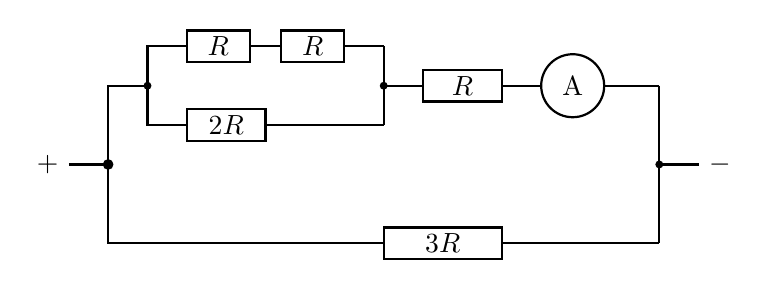
\begin{tikzpicture}[>=stealth, thick]
    % Kirish terminali (+)
    \draw (0,1) -- (0.5,1);
    \node[left] at (0,1) {$+$};
    \filldraw (0.5,1) circle (1.5pt);

    % Asosiy tarmoqlanish (Yuqori va pastki tarmoq)
    \draw (0.5,1) -- (0.5,2) -- (1,2); % Yuqori katta tarmoqqa
    \draw (0.5,1) -- (0.5,0) -- (4,0); % Pastki tarmoqqa (3R)

    % Yuqori tarmoq ichidagi parallel blok (R+R va 2R)
    \filldraw (1,2) circle (1pt);
    \draw (1,2) -- (1,2.5) -- (1.5,2.5); % R+R yo'li
    \draw (1,2) -- (1,1.5) -- (1.5,1.5); % 2R yo'li

    % R va R ketma-ket (eng yuqorida)
    \draw (1.5,2.3) rectangle (2.3,2.7) node[midway] {$R$};
    \draw (2.3,2.5) -- (2.7,2.5);
    \draw (2.7,2.3) rectangle (3.5,2.7) node[midway] {$R$};
    \draw (3.5,2.5) -- (4,2.5);

    % 2R rezistori (o'rtada)
    \draw (1.5,1.3) rectangle (2.5,1.7) node[midway] {$2R$};
    \draw (2.5,1.5) -- (4,1.5);

    % Parallel blokning birlashishi va davomi (R va A)
    \draw (4,2.5) -- (4,1.5);
    \filldraw (4,2) circle (1pt);
    \draw (4,2) -- (4.5,2);
    \draw (4.5,1.8) rectangle (5.5,2.2) node[midway] {$R$};
    \draw (5.5,2) -- (6,2);
    \draw (6.4,2) circle (0.4) node {A};
    \draw (6.8,2) -- (7.5,2);

    % Pastki tarmoqdagi 3R rezistori
    \draw (4, -0.2) rectangle (5.5, 0.2) node[midway] {$3R$};
    \draw (5.5,0) -- (7.5,0);

    % Yakuniy birlashish va chiqish terminali (-)
    \draw (7.5,2) -- (7.5,0);
    \filldraw (7.5,1) circle (1pt);
    \draw (7.5,1) -- (8,1);
    \node[right] at (8,1) {$-$};

\end{tikzpicture}

\begin{enumerate}[label=\Alph*)]
\item 15.
\item 25.
\item 20.
\item 30.
\item 10.
\end{enumerate}

\item Suv qaynatkich elektr asbob spiralining qarshiligi $100^\circ$C temperaturada $22~\Omega$. $100^\circ$C temperaturadagi $360$ g suvni $6$ minutda bug‘ga aylantirish uchun bu spiral orqali qanday tok o‘tkazish kerak (A)? Suvning solishtirma bug‘lanish issiqligi $2200$ kJ/kg.
\begin{enumerate}[label=\Alph*)]
\item 1,5.
\item 10.
\item 15.
\item 18.
\item 19.
\end{enumerate}

\item Qarshiligi $330~\Omega$ bo‘lgan isitkichdan o‘tayotgan tokning kuchi necha Amper bo‘lganda $0^\circ$C temperaturali $1$ g muz $1$ s da eriydi? Muzning solishtirma erish issiqligi $3,3\cdot10^5$ J/kg.
\begin{enumerate}[label=\Alph*)]
\item 5.
\item 3,6.
\item 0,33.
\item 0,5.
\item 1.
\end{enumerate}

\item Qarshiligi $16,8$ k$\Omega$ bo‘lgan isitkichda necha Amper tok kuchi $1$ s da $10$ g suvni erish nuqtasidan qaynash nuqtasigacha isitadi? Suvning solishtirma issiqlik sig‘imi $4,2$ kJ/(kg$\cdot$K).
\begin{enumerate}[label=\Alph*)]
\item 4.
\item 2,5.
\item 2.
\item 0,5.
\item 0,25.
\end{enumerate}

\item Quyidagi elektr zanjirda kalit uzuq va suvning temperaturasi $40^\circ$C. Kalit ulansa necha minutdan so‘ng suvning temperaturasi $70^\circ$C ga yetadi? $c=4200$ J/kg$\cdot$K.

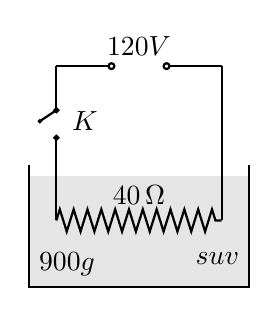
\begin{tikzpicture}[>=stealth, thick, scale=0.7]
    % Kuchlanish manbai terminallari (yuqorida)
    \draw (1.5,4) -- (2.45,4);
    \draw (3.55,4) -- (4.5,4);
    \draw (2.5,4) circle (1.5pt);
    \draw (3.5,4) circle (1.5pt);
    \node[above] at (3,4) {$120 \text{ V}$};

    % Chap tomondagi sim va K kaliti
    \draw (1.5,4) -- (1.5,3.2);
    \draw (1.5,2.7) -- (1.5,1.5);
    \draw (1.5,3.2) -- (1.2, 3) circle (0.5pt); % Kalitning harakatlanuvchi qismi
    \filldraw (1.5,3.2) circle (1pt);
    \filldraw (1.5,2.7) circle (1pt);
    \node[right] at (1.6,3) {$K$};

    % O'ng tomondagi sim
    \draw (4.5,4) -- (4.5,1.5);

    % Suvli idish (shisha yoki metall idish tasviri)
    \fill[gray!20] (1,0) rectangle (5,2); % Suv sathi
    \draw (1,2.2)--(1,0) -- (5,0) -- (5,2.2);
    
    % Isitkich spirali (40 Ohm)
    \draw (1.5,2) -- (1.5,1.2);
    \draw (4.5,2) -- (4.5,1.2);
    \draw[decorate, decoration={zigzag, segment length=5pt, amplitude=4pt}] (1.5,1.2) -- (4.5,1.2);
    \node[above] at (3,1.3) {$40 \, \Omega$};

    % Idish ichidagi yozuvlar
    \node[below right] at (1,0.8) {$900 \text{ g}$};
    \node[below left] at (5,0.8) {$\text{suv}$};

\end{tikzpicture}

\begin{enumerate}[label=\Alph*)]
\item 4,2.
\item 5,25.
\item 6,5.
\item 8,3.
\item 10,48.
\end{enumerate}

\item Chulg‘amning qarshiligi $50~\Omega$ bo‘lgan elektrchoynakda temperaturasi $0^\circ$C bo‘lgan $600$ cm$^3$ suv bor. Agar tarmoq kuchlanishi $200$ V, choynakning FIK $60\%$ bo‘lsa, undagi hamma suvni qaynatib, bug‘ga aylantirish uchun necha minut vaqt kerak bo‘ladi? Suv uchun $c=4,2$ kJ/(kg$\cdot$K), $r=2,3$ MJ/kg.
\begin{enumerate}[label=\Alph*)]
\item 57.
\item 28.
\item 32.
\item 41.
\item 50.
\end{enumerate}

\item Qaysi qarshilikda eng ko‘p issiqlik ajraladi? $R_1=1~\Omega$, $R_2=R_3=2~\Omega$, $R_4=4~\Omega$.

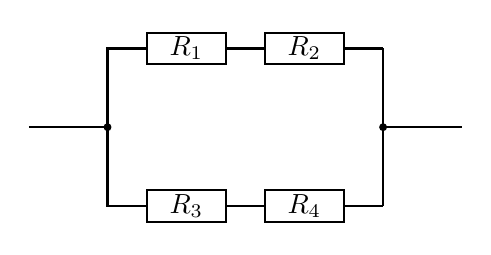
\begin{tikzpicture}[>=stealth, thick]
    % Chap tomondagi kirish simi
    \draw (0,0) -- (1,0);
    \filldraw (1,0) circle (1pt);

    % Tarmoqlanish (Parallel blok boshlanishi)
    \draw (1,0) -- (1,1) -- (1.5,1);   % Yuqori tarmoqqa
    \draw (1,0) -- (1,-1) -- (1.5,-1); % Pastki tarmoqqa

    % Yuqori tarmoq: R1 va R2 ketma-ket
    \draw (1.5,0.8) rectangle (2.5,1.2) node[midway] {$R_1$};
    \draw (2.5,1) -- (3,1);
    \draw (3,0.8) rectangle (4,1.2) node[midway] {$R_2$};
    \draw (4,1) -- (4.5,1);

    % Pastki tarmoq: R3 va R4 ketma-ket
    \draw (1.5,-1.2) rectangle (2.5,-0.8) node[midway] {$R_3$};
    \draw (2.5,-1) -- (3,-1);
    \draw (3,-1.2) rectangle (4,-0.8) node[midway] {$R_4$};
    \draw (4,-1) -- (4.5,-1);

    % Birlashish (Parallel blok oxiri)
    \draw (4.5,1) -- (4.5,0);
    \draw (4.5,-1) -- (4.5,0);
    \filldraw (4.5,0) circle (1pt);
    \draw (4.5,0) -- (5.5,0); % Chiqish simi

\end{tikzpicture}

\begin{enumerate}[label=\Alph*)]
\item $R_1$ da.
\item $R_2$ da.
\item $R_3$ da.
\item $R_4$ da.
\item hammasida bir xil.
\end{enumerate}

\item Qarshiligi $R_1$ bo‘lgan qaynatgich biror miqdor suvni $t_1$ vaqtda qaynatadi. Qarshiligi $R_2$ bo‘lgan qaynatgich esa shu sharoitda o‘sha suvni $t_2$ vaqtda qaynatadi. Ikkala qaynatgich parallel ulansa o‘sha suv qanday vaqtda qaynaydi?
\begin{enumerate}[label=\Alph*)]
\item $t_1+t_2$.
\item $\dfrac{t_1t_2}{t_1+t_2}$.
\item $\sqrt{t_1t_2}$.
\item $\dfrac{t_1+t_2}{2}$.
\item $\dfrac{2t_1t_2}{t_1+t_2}$.
\end{enumerate}

\item Elektr choynakda ikkita chulg‘am bor. Birinchi chulg‘am ulanganda, suv $t_1$ vaqtda, ikkinchisi ulanganda, $t_2$ vaqtda qaynaydi. Ikkala chulg‘am ketma-ket ulanganda qaynash vaqti, ular parallel ulangandagi qaynash vaqtidan necha marta katta bo‘ladi?
\begin{enumerate}[label=\Alph*)]
\item $\dfrac{2t_1t_2}{t_1+t_2}$.
\item $\dfrac{t_1+t_2}{t_1t_2}$.
\item $\dfrac{(t_1+t_2)^2}{t_1t_2}$.
\item $\dfrac{t_1-t_2}{t_1+t_2}$.
\item $\dfrac{t_1t_2}{t_1+t_2}$.
\end{enumerate}

\item Ikkita bir xil elektr plita parallel ulansa, suv $t$ vaqtda qaynaydi. Shu plitalar ketma-ket ulanganida suv qancha vaqtda qaynaydi?
\begin{enumerate}[label=\Alph*)]
\item $2t$.
\item $t/2$.
\item $t/3$.
\item $4t$.
\item $1,5t$.
\end{enumerate}

\end{enumerate}

